% +++++++++++++++++++++++++++++++++++++++++++++++++++++++++++
% University of Southern Maine
% Department of Computer Science
% Discrete Mathematics II (COS 280)
% James Quinlan (https://cs.usm.maine.edu/~james.quinlan/)
% Homework Template
% +++++++++++++++++++++++++++++++++++++++++++++++++++++++++++

% EDIT Lines: 11, 12, 13
\def\filename{Master Theorem}   		   % included file (edit file)
\def\chapsec{Appendix B.4}  % Chapter/Section/Topic
\def\yourname{Master Theorem}	   % Your name
\def\course{COS 485}		   % Course (if different)

% ---------------- Do NOT Edit Below ------------------------
% -----------------------------------------------------------
\documentclass[11pt]{article}

\def\pf{\textit{Proof}: }

\usepackage{amsfonts}
\usepackage{amssymb}
\usepackage{amstext}
\usepackage{amscd}
\usepackage{amsmath}
\usepackage{xspace}
\usepackage{theorem}
\usepackage{float}
\usepackage[table]{xcolor}
\usepackage{color}
\usepackage{soul}
\usepackage{booktabs}
\usepackage{outlines}
\usepackage{enumitem}
\usepackage{algorithm}
\usepackage{algpseudocode}
\usepackage{pgf-pie}
\usepackage{fancybox}
\usepackage{mathtools}
\usepackage{circuitikz}
\setenumerate[1]{label=\arabic*.}
\setenumerate[2]{label=(\alph*).}
\setenumerate[3]{label=\roman*.}
\setenumerate[4]{label=\alph*.}

\usepackage{hyperref}
\hypersetup{
    colorlinks=true,
    linkcolor=blue,
    filecolor=magenta,      
    urlcolor=cyan,
    pdftitle={\filename},
    pdfpagemode=FullScreen,
    }

% TikZ
\usepackage{tikz}
\usepackage{pgfplots}
\pgfplotsset{compat=1.15}
\usepackage{mathrsfs}
\usetikzlibrary{arrows}

% Colors
\definecolor{stainlessSteel}{cmyk}{0,0,0.02,0.12}

% Document Geometry
\makeatletter
 \setlength{\textwidth}{6.75in}
 \setlength{\oddsidemargin}{0in}
 \setlength{\evensidemargin}{0in}
 \setlength{\topmargin}{0.0125in}
 \setlength{\textheight}{9.0in}
 \setlength{\headheight}{0pt}
 \setlength{\headsep}{0pt}
 \setlength{\marginparwidth}{59pt}

 \setlength{\parindent}{0pt}
 \setlength{\parskip}{5pt plus 1pt}
 \setlength{\theorempreskipamount}{5pt plus 1pt}
 \setlength{\theorempostskipamount}{0pt}
 \setlength{\abovedisplayskip}{8pt plus 3pt minus 6pt}
 \setlength{\intextsep}{15pt plus 3pt minus 6pt}

 % Headings
 \renewcommand{\section}{\@startsection{section}{1}{0mm}%
    {2ex plus -1ex minus -.2ex}%
    {1.3ex plus .2ex}%
    {\normalfont\Large\bfseries}}%
 \renewcommand{\subsection}{\@startsection{subsection}{2}{0mm}%
    {1ex plus -1ex minus -.2ex}%
    {1ex plus .2ex}%
    {\normalfont\large\bfseries}}%
 \renewcommand{\subsubsection}{\@startsection{subsubsection}{3}{0mm}%
    {1ex plus -1ex minus -.2ex}%
    {1ex plus .2ex}%
    {\normalfont\normalsize\bfseries}}
 \renewcommand\paragraph{\@startsection{paragraph}{4}{0mm}%
    {1ex \@plus1ex \@minus.2ex}%
    {-1em}%
    {\normalfont\normalsize\bfseries}}
 \renewcommand\subparagraph{\@startsection{subparagraph}{5}{\parindent}%
    {2.0ex \@plus1ex \@minus .2ex}%
    {-1em}%
    {\normalfont\normalsize\bfseries}}
\makeatother

\newcounter{thelecture}

\newenvironment{proof}{{\bf Proof:  }}{\hfill\rule{2mm}{2mm}}
\newenvironment{proofof}[1]{{\bf Proof of #1:  }}{\hfill\rule{2mm}{2mm}}
\newenvironment{proofofnobox}[1]{{\bf#1:  }}{}
\newenvironment{example}{{\bf Example: }}{\hfill\rule{0mm}{0mm}} % change 2mm 2mm for square

%\renewcommand{\theequation}{\thesection.\arabic{equation}}
%\renewcommand{\thefigure}{\thesection.\arabic{figure}}

\newtheorem{fact}{Fact}
\newtheorem{lemma}[fact]{Lemma}
\newtheorem{theorem}[fact]{Theorem}
\newtheorem{definition}[fact]{Definition}
\newtheorem{corollary}[fact]{Corollary}
\newtheorem{proposition}[fact]{Proposition}
\newtheorem{claim}[fact]{Claim}
\newtheorem{exercise}[fact]{Exercise}

% math notation
\newcommand{\R}{\ensuremath{\mathbb R}}
\newcommand{\Z}{\ensuremath{\mathbb Z}}
\newcommand{\N}{\ensuremath{\mathbb N}}
\newcommand{\B}{\ensuremath{\mathbb B}}
\newcommand{\F}{\ensuremath{\mathcal F}}
\newcommand{\SymGrp}{\ensuremath{\mathfrak S}}
\newcommand{\prob}[1]{\ensuremath{\text{{\bf Pr}$\left[#1\right]$}}}
\newcommand{\expct}[1]{\ensuremath{\text{{\bf E}$\left[#1\right]$}}}
\newcommand{\size}[1]{\ensuremath{\left|#1\right|}}
\newcommand{\ceil}[1]{\ensuremath{\left\lceil#1\right\rceil}}
\newcommand{\floor}[1]{\ensuremath{\left\lfloor#1\right\rfloor}}
\newcommand{\ang}[1]{\ensuremath{\langle{#1}\rangle}}
\newcommand{\poly}{\operatorname{poly}}
\newcommand{\polylog}{\operatorname{polylog}}

% Anupam's abbreviations
\newcommand{\e}{\epsilon}
\newcommand{\half}{\ensuremath{\frac{1}{2}}}
\newcommand{\junk}[1]{}
\newcommand{\sse}{\subseteq}
\newcommand{\union}{\cup}
\newcommand{\meet}{\wedge}
\newcommand{\dist}[1]{\|{#1}\|_{\text{dist}}}
\newcommand{\hooklongrightarrow}{\lhook\joinrel\longrightarrow}
\newcommand{\embeds}[1]{\;\lhook\joinrel\xrightarrow{#1}\;}
\newcommand{\mnote}[1]{\normalmarginpar \marginpar{\tiny #1}}



% -----------------------------------------------------------
% Header
\newcommand{\hwheadings}[3]{
{\chapsec } \hfill {{ \yourname }} \hfill {{ \course #1}}\\
{{\bf } #2} \hfill { #3} 
\rule[0.051in]{\textwidth}{0.0025in}
%\thispagestyle{empty}
}

% Document begins here 
\begin{document}
\hwheadings{}{}{}
filler % causes a warning if no text here
\section*{\centering Master Theorem}

\section*{Overview}

\begin{outline}[enumerate]
  \1 Theorem 
  \1 Proof
  \1 Examples 
\end{outline}

\section*{Theorem}%
\label{sec:theorem}

Suppose a complexity function $T(n)$ is eventually non-decreasing and satisfies

\begin{align*}
  &T(n) = aT\left(\frac{n}{b}\right) + O(n^d) & \textrm{for } n > 1 \textrm{, } n \textrm{ a power of } b \\
  &T(1) = c
\end{align*}


Where $b \ge 2$ and $d \ge 0$ are constant \textit{integers}, and $a$ and $c$ are constant such that 
$a > 0$ and $c > 0$. Then
\[
  T(n) \in 
  \begin{cases}
    \Theta(n^d) & \textrm{if } a < b^d \\
    \Theta(n^d \lg n) & \textrm{if } a = b^d \\
    \Theta(n^{\log_{b} a}) & \textrm{if } a > b^d
  \end{cases}
\] 

Also, using the same theorem, if in the recurrence relation

\[
  T(n) = aT\left(\frac{n}{b}\right) + O(n^d) 
\] 
the equality is replaced by an inequality, such as 

\begin{align*}
  T(n) \le aT\left(\frac{n}{b}\right) + O(n^d) 
  & & \textrm{or} & &
  T(n) \ge aT\left(\frac{n}{b}\right) + O(n^d)
\end{align*}

Then the results above hold true with ``big $O$'' or  $\Omega$, respectively, replacing $\Theta$
\section*{Proof}%
\label{sec:proof}

It is important to understand the different parts of the recurrence relation used in the theorem.

\[
  \underbrace{T(n)}_{\mathclap{\textrm{Recurrence relation}}} = 
  \overbrace{a}^{\mathclap{\textrm{Subproblems}}}
  T\underbrace{\left(\frac{n}{b}\right)}_{\textrm{Divisor}}
  + O(n^{\overbrace{d}^{\mathclap{\textrm{Degree of work time complexity}}}})
\] 

The general solution to the recurrence relation above can be described as
\[
  T(n) = \sum_{i=0}^{\log_{b} n} O\left(n^d\right) \left(\frac{a}{b^d}\right)^i
\] 

This can be visually seen by drawing the recursion tree generated by the relation shown above.
The tree has a \textit{depth} of $\log_{b} n$ and a \textit{branching factor} of $a$. At level  $i$,
there are  $a^i$ nodes each with a work of $O\left(\frac{n}{b}\right)^d$. The value of the relation
is the sum of all the nodes on the tree. The sum is found by summing the work from all
$\log_{b} n$ levels.

\begin{figure}[!ht]
\label{fig:master-thm}
\centering
\resizebox{1\textwidth}{!}{%
\begin{circuitikz}

% Top
\draw [dashed] (1,15.25) -- (24.5,15.25);
\node [font=\LARGE] at (1.75,15.75) {Level};
\node [font=\LARGE] at (10,15.75) {Size of Problem};
\node [font=\LARGE] at (19,15.75) {Subproblems};
\node [font=\LARGE] at (22.75,15.75) {Work};

% Levels
\draw [dashed] (2.75,16.25) -- (2.75,4.75);
\node [font=\LARGE] at (1.75,14.25) {$0$};
\node [font=\LARGE] at (1.75,12.25) {$1$};
\node [font=\LARGE] at (1.75,10.25) {$i$};
\node [font=\LARGE, rotate around={90:(0,0)}] at (1.75,8.75) {$...$};
\node [font=\LARGE] at (1.75,6.5) {$\log_b n$};

% Size
\draw [dashed] (17,16.25) -- (17,4.75);
\draw  (9.5,15) rectangle  node {\LARGE $n$} (10.5,14);
\draw [->, >=Stealth] (9.5,14) -- (7,13);
\draw [->, >=Stealth] (10.5,14) -- (13,13);

\draw  (6,13) rectangle  node {\LARGE $\frac{n}{b}$} (7,12);
\draw  (13,13) rectangle  node {\LARGE $\frac{n}{b}$} (14,12);
\draw [->, >=Stealth, dashed] (6,12) -- (5.25,10.5);
\draw [->, >=Stealth, dashed] (7,12) -- (7.75,10.5);
\draw [->, >=Stealth, dashed] (13,12) -- (12.25,10.5);
\draw [->, >=Stealth, dashed] (14,12) -- (14.75,10.5);

\draw  (4.25,10.5) rectangle  node {\huge $\frac{n}{b^i}$} (5.25,9.5);
\draw  (7.75,10.5) rectangle  node {\huge $\frac{n}{b^i}$} (8.75,9.5);
\draw  (14.75,10.5) rectangle  node {\huge $\frac{n}{b^i}$} (15.75,9.5);
\draw  (11.25,10.5) rectangle  node {\huge $\frac{n}{b^i}$} (12.25,9.5);

\node [font=\LARGE, rotate around={90:(0,0)}] at (4.75,8.75) {$...$};
\node [font=\LARGE, rotate around={90:(0,0)}] at (8.25,8.75) {$...$};
\node [font=\LARGE, rotate around={90:(0,0)}] at (11.75,8.75) {$...$};
\node [font=\LARGE, rotate around={90:(0,0)}] at (15.25,8.75) {$...$};
\draw [->, >=Stealth, dashed] (4.75,8.25) -- (4.25,7);
\draw [->, >=Stealth, dashed] (4.75,8.25) -- (5.25,7);
\draw [->, >=Stealth, dashed] (8.25,8.25) -- (7.75,7);
\draw [->, >=Stealth, dashed] (8.25,8.25) -- (8.75,7);
\draw [->, >=Stealth, dashed] (11.75,8.25) -- (11.25,7);
\draw [->, >=Stealth, dashed] (11.75,8.25) -- (12.25,7);
\draw [->, >=Stealth, dashed] (15.25,8.25) -- (14.75,7);
\draw [->, >=Stealth, dashed] (15.25,8.25) -- (15.75,7);

\draw  (3.25,7) rectangle  node {\large $1$} (4.25,6);
\draw  (5.25,7) rectangle  node {\large $1$} (6.25,6);
\draw  (6.75,7) rectangle  node {\large $1$} (7.75,6);
\draw  (8.75,7) rectangle  node {\large $1$} (9.75,6);
\draw  (10.25,7) rectangle  node {\large $1$} (11.25,6);
\draw  (12.25,7) rectangle  node {\large $1$} (13.25,6);
\draw  (13.75,7) rectangle  node {\large $1$} (14.75,6);
\draw  (15.75,7) rectangle  node {\large $1$} (16.75,6);

% Subproblems
\draw [dashed] (21,16.25) -- (21,4.75);
\node [font=\LARGE] at (19,14.5) {$a$};
\node [font=\LARGE] at (19,12.75) {$a^1$};
\node [font=\LARGE] at (19,10) {$a^i$};
\node [font=\LARGE] at (19,6.5) {$a^{\log_b n}$};

% Work
\node [font=\LARGE] at (22.75,14.5) {$O(n^d)$};
\node [font=\LARGE] at (22.75,13) {$a \cdot O\left(\frac{n}{b}\right)^d $};
\node [font=\LARGE] at (22.75,11.75) {$= O(n^d) \cdot \frac{a}{b^d}$};
\node [font=\LARGE] at (22.75,10.25) {$a^i \cdot O\left(\frac{n}{b^i}\right)^d$};
\node [font=\LARGE] at (23,9) {$= O(n^d) \cdot \left(\frac{a}{b^d}\right)^i$};
\node [font=\LARGE] at (22.75,6.75) {$a^{\log_{b} n} \cdot O(1)$};
\node [font=\LARGE] at (22.75,5.5) {$= O\left(n^{\log_{b} a}\right)  $};

% Total
\node [font=\LARGE] at (17.5,3) {Total Work = };
\node [font=\LARGE] at (21.75,3) {$\sum_{i=0}^{\log _{b} n} O\left(n^d\right) \left(\frac{a}{b^d}\right)^i$};

\end{circuitikz}
}%
\end{figure}

Now that the solution is found, let's address the three cases shown in the theorem.

\subsection*{Case One}%
\label{sub:case-one}

\[
  T(n) \in \Theta \left(n^d\right) \iff a < b^d \textrm{, or } d > \log_{b} a
.\]

For case one we will use substitution.

\[
  \sum_{i=0}^{\log_{b}n} \underbrace{O(n^d)}_{\textrm{\large a}} \underbrace{\left(\frac{a}{b^d}\right)^i}_{\textrm{\large r}} = O(n^d) \iff \left(\frac{a}{b^d}\right)^i < 1
\] 
\pf
\begin{align*}
  \sum_{i=0}^{n-1} ar^i &= ar^0 + ar + ar^2 + ar^3 + \cdots + ar^{n-1} \\
  &= a\left(\frac{1-r^n}{1-r}\right) & r \neq 1 \\
  & r > 1 \textrm{ or } r < 1  & = \begin{cases}
    O(a), & r < 1 \\
    O(ar^{n-1}), & r > 1 \\
  \end{cases} \\ 
  \sum_{i=0}^{n-1} ar^i &\le O(a) \iff r < 1 \\
  \sum_{i=0}^{n-1} ar^i &\le O(ar^{n-1}) \iff r > 1 \\
\end{align*}

\subsection*{Case Two}%
\label{sub:Case Two}

\[
  T(n) \in \Theta \left(n^d \lg n\right) \iff a = b^d \textrm{, or } d = \log_{b} a
\] 
\pf
\begin{align*}
  \frac{a}{b^d} = 1 \iff d &= \log_{b} a \\
  \sum_{i=0}^{\log_{b} n} O(n^d)\left(\frac{a}{b^d}\right)^i &= \sum_{i=0}^{\log_{b} n} O(n^d) \\ 
  &=(\log_{b} n+1) \cdot O(n^d) \\
  &=(\log_{b} n) \cdot O(n^d) + \underbrace{O(n^d)}_{\mathclap{\textrm{lower order term}}}\\
  &=\log_{b} n \cdot O(n^d) \\
  &=O\left(n^d \cdot \frac{\log n}{\log b}\right) \\
  &=O\left(n^d \lg n \right) \\
\end{align*}


\subsection*{Case Three}%
\label{sub:Case Three}

\[
  T(n) \in \Theta \left(n^{\log_{b} n}\right) \iff a > b^d \textrm{, or } d < \log_{b} a
.\] 

\pf
\begin{align*}
  \frac{a}{b^d} > 1 \iff d &< \log_{b} a \\
  \sum_{i=0}^{\log_{b} n} O(n^d)\left(\frac{a}{b^d}\right)^i &= O\left(O(n^d) \cdot \left(\frac{a}{b^d}\right)^{\log_{b} n}\right)\\ 
  &= O\left(O(n^d) \cdot \frac{a^{\log_{b} n}}{(b^d)^{\log_{b} n}}\right)\\ 
  &= O\left(O(n^d) \cdot \frac{n^{\log_{b} a}}{b^{\log_{b} n^d}}\right)\\ 
  &= O\left(O(n^d) \cdot \frac{n^{\log_{b} a}}{n^d}\right)\\ 
  &= O\left(\frac{Cn^d}{n^d}\cdot n^{\log_{b} a}\right)\\ 
  &= O\left(n^{\log_{b} a}\right)\\ 
\end{align*}

\section*{Examples}%
\label{sec:examples}

\subsection*{Merge Sort}%
\label{sub:Merge Sort}

Merge Sort is a recursive algorithm, the time complexity can be expressed with the following recurrence relation.

\[
  T(n) = \underbrace{2}_{a}T \underbrace{\left(\frac{n}{2}\right)}_{b} + \underbrace{O(n)}_{d = 1}
\] 

Using the Master Theorem we get

\begin{align*}
  &a = 2 &  b = 2 & & d = 1 \\ 
\end{align*}

Which means the middle case holds true for Merge Sort

\[
  T(n) \in 
  \begin{cases}
    \Theta(n^d) & \textrm{if } a < b^d \\
    \Theta(n^d \lg n) & \textrm{if } a = b^d \\
    \Theta(n^{\log_{b} a}) & \textrm{if } a > b^d
  \end{cases}
\] 
\begin{align*}
  &a = b^d & 2 = 2^1 \\ 
\end{align*}
\[
  T(n) \in \Theta(n \lg n)
.\] 
The proof of this can be seen visually with the diagram below

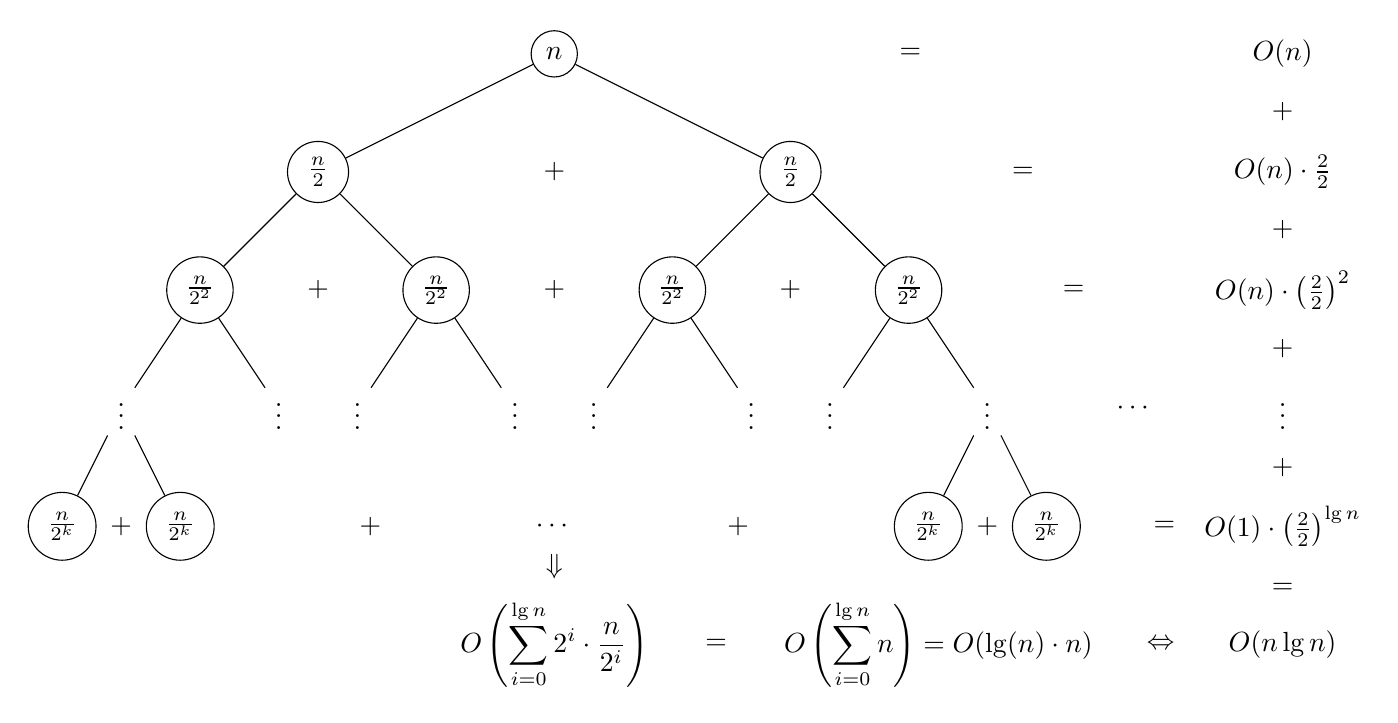
\begin{tikzpicture}[level/.style={sibling distance=60mm/#1}]
  \node [circle,draw] (z){$n$}
    child {node [circle,draw] (a) {$\frac{n}{2}$}
      child {node [circle,draw] (b) {$\frac{n}{2^2}$}
        child {node {$\vdots$}
          child {node [circle,draw] (d) {$\frac{n}{2^k}$}}
          child {node [circle,draw] (e) {$\frac{n}{2^k}$}}
        } 
        child {node {$\vdots$}}
      }
      child {node [circle,draw] (g) {$\frac{n}{2^2}$}
        child {node {$\vdots$}}
        child {node {$\vdots$}}
      }
    }
    child {node [circle,draw] (j) {$\frac{n}{2}$}
      child {node [circle,draw] (k) {$\frac{n}{2^2}$}
        child {node {$\vdots$}}
        child {node {$\vdots$}}
      }
    child {node [circle,draw] (l) {$\frac{n}{2^2}$}
      child {node {$\vdots$}}
      child {node (c){$\vdots$}
        child {node [circle,draw] (o) {$\frac{n}{2^k}$}}
        child {node [circle,draw] (p) {$\frac{n}{2^k}$}
          child [grow=right] {node (q) {$=$} edge from parent[draw=none]
            child [grow=right] {node (q) {$O(1) \cdot \left(\frac{2}{2}\right)^{\lg n}$} edge from parent[draw=none]
              child [grow=up] {node (r) {$\vdots$} edge from parent[draw=none]
                child [grow=up] {node (s) {$O(n) \cdot \left(\frac{2}{2}\right)^2$} edge from parent[draw=none]
                  child [grow=up] {node (t) {$O(n) \cdot \frac{2}{2}$} edge from parent[draw=none]
                    child [grow=up] {node (u) {$O(n)$} edge from parent[draw=none]}
                  }
                }
              }
              child [grow=down] {node (v) {$O(n \lg n)$}edge from parent[draw=none]}
            }
          }
        }
      }
    }
  };
  \path (a) -- (j) node [midway] {+};
  \path (b) -- (g) node [midway] {+};
  \path (k) -- (l) node [midway] {+};
  \path (k) -- (g) node [midway] {+};
  \path (d) -- (e) node [midway] {+};
  \path (o) -- (p) node [midway] {+};
  \path (o) -- (e) node (x) [midway] {$\cdots$}
    child [grow=down] {
      node (y) {$O\left(\displaystyle\sum_{i = 0}^{\lg n} 2^i \cdot \frac{n}{2^i}\right)$}
      edge from parent[draw=none]
    };
  \path (q) -- (r) node [midway] {+};
  \path (s) -- (r) node [midway] {+};
  \path (s) -- (t) node [midway] {+};
  \path (s) -- (l) node [midway] {=};
  \path (t) -- (u) node [midway] {+};
  \path (z) -- (u) node [midway] {=};
  \path (j) -- (t) node [midway] {=};
  \path (y) -- (x) node [midway] {$\Downarrow$};
  \path (v) -- (y)
    node (w) [midway] {$O\left(\displaystyle\sum_{i = 0}^{\lg n} n\right) = O(\lg(n) \cdot n)$};
  \path (q) -- (v) node [midway] {=};
  \path (e) -- (x) node [midway] {+};
  \path (o) -- (x) node [midway] {+};
  \path (y) -- (w) node [midway] {$=$};
  \path (v) -- (w) node [midway] {$\Leftrightarrow$};
  \path (r) -- (c) node [midway] {$\cdots$};
\end{tikzpicture}

\subsection*{Other Examples}%
\label{sub:Other Examples}

Consider the following recurrence relation

\[
  T(n) = \underbrace{9}_{a} T(n / \underbrace{3}_{b} ) + 5n^{\overbrace{1}^{d}}
\] 

By the Master Theorem, using case 3, because $9 > 3^1$

\[
  T(n) \in \Theta\left(n^{\log_{3} 9}\right) = \Theta(n^2)
.\] 
\hrule

Consider the following recurrence relation

\[
  T(n) = \underbrace{3}_{a} T(n/\underbrace{2}_{b}) + 3n^{\overbrace{3}^{d}} + 2n^2 
.\] 
By the Master Theorem, using case 1, because $3 < 2^3$

\[
  T(n) \in \Theta(n^3)
.\]

\end{document}
% -----------------------------------------------------------
